\documentclass[letterpaper, 10 pt, conference]{ieeeconf}  % Comment this line out if you need a4paper

%\documentclass[a4paper, 10pt, conference]{ieeeconf}      % Use this line for a4 paper

\IEEEoverridecommandlockouts                              % This command is only needed if 
                                                          % you want to use the \thanks command

\overrideIEEEmargins                                      % Needed to meet printer requirements.

%In case you encounter the following error:
%Error 1010 The PDF file may be corrupt (unable to open PDF file) OR
%Error 1000 An error occurred while parsing a contents stream. Unable to analyze the PDF file.
%This is a known problem with pdfLaTeX conversion filter. The file cannot be opened with acrobat reader
%Please use one of the alternatives below to circumvent this error by uncommenting one or the other
%\pdfobjcompresslevel=0
%\pdfminorversion=4

% See the \addtolength command later in the file to balance the column lengths
% on the last page of the document

% The following packages can be found on http:\\www.ctan.org
%\usepackage{graphics} % for pdf, bitmapped graphics files
%\usepackage{epsfig} % for postscript graphics files
%\usepackage{mathptmx} % assumes new font selection scheme installed
%\usepackage{times} % assumes new font selection scheme installed
%\usepackage{amsmath} % assumes amsmath package installed
\usepackage{amssymb}  % assumes amsmath package installed
\usepackage{amscd,amsmath}
\usepackage{amsfonts}
\usepackage{biblatex}
\usepackage{csvsimple}
\usepackage{pgfplots}
\usepackage{pgfplotstable}
\usepackage{hyperref}
\usepackage{algorithm}
\usepackage{algpseudocode}
\usepackage{rotating}
\usepackage{gensymb}
%\pgfplotsset{compat=1.7}
\usepackage{graphicx}
\usepackage{import}
\usepackage{placeins}
\usepackage{multirow}
\usepackage{booktabs}
\usepackage{xcolor}
\usepackage{pgf}
\usepackage{subcaption}
%\usepackage[maxfloats=256]{morefloats}
%\maxdeadcycles=1000
%\usepgfplotslibrary{external} 
%\tikzexternalize

\newcommand\norm[1]{\left\lVert#1\right\rVert}

\title{\LARGE \bf
Fault Detection of Sun Reflection to Increase Estimation Accuracy of Satellite Attitude
}


\author{Louw UJ$^{1}$, Jordaan HW$^{2}$, Schoeman JC$^{3}$% <-this % stops a space
\thanks{*This work was not supported by any organization}% <-this % stops a space
\thanks{$^{1}$Louw UJ is with Faculty of Electronic \& Electrical Engineering, Electronic System            Laboratory, University of Stellenbosch, Stellenbosch Central, Stellenbosch, 7600
        {\tt\small louwuj@gmail.com}}%
}

\addbibresource{bibliography.bib} 

\begin{document}



\maketitle
\thispagestyle{empty}
\pagestyle{empty}


%%%%%%%%%%%%%%%%%%%%%%%%%%%%%%%%%%%%%%%%%%%%%%%%%%%%%%%%%%%%%%%%%%%%%%%%%%%%%%%%
\begin{abstract}

The Kalman Filter is a state estimator often used in attitude determination of satellites. A Kalman filter is susceptible to anomalies that occur in sensors. An excellent example of this is the reflection of a solar panel on a sun sensor that changes the perceived sun vector. Sun reflection in term influences the estimation of the attitude by the Kalman filter and, consequently, the satellite's control. Detecting anomalies in sensors and omitting the sensor reading from the measurement update of the Kalman Filter increases the stability and reliability of the Kalman filter for satellite attitude determination. However, detecting when an anomaly occurs is challenging, and an accuracy of more than $99\%$ is required to produce satisfactory results unless only the two sensors with the smallest error between the estimated vector and the measured vector is used during a fixed period after the fault is detected. This then decreases the required accuracy to $70\%$.

\end{abstract}

%%%%%%%%%%%%%%%%%%%%%%%%%%%%%%%%%%%%%%%%%%%%%%%%%%%%%%%%%%%%%%%%%%%%%%%%%%%%%%%%
\section{INTRODUCTION}
For many satellite missions, attitude determination is of high importance. For example, a mission that requires earth following during eclipse and otherwise sun following for solar charging requires accurate attitude estimation. However, the current state vector of the system can not be determined with only the use of models or sensors. Since the sensors contain noise and the mathematical model does not include certain disturbances of the existing system. Therefore a probabilistic approach can determine the attitude from both the model and the sensors, for which we generally use an extended Kalman filter (\emph{EKF}).

The attitude determination and control system, \emph{ADCS}, of the satellite is demonstrated in Figure~\ref{fig:System_Diagram}, where the basic ADCS excludes fault detection, isolation and recovery, \emph{FDIR}, and feature extraction. The FDIR for sensors receive the sensor measurements and the feature extractions as inputs and outputs the recovery method when required. 

The EKF is a method that incorporates a physics-based model of the satellite dynamics with sensor fusion and measurement updates to ensure accurate estimation. The sensor measurements used for the measurement update are the sensors that provide a modelled vector in the orbit-referenced coordinate, \emph{ORC}, frame, and a measured vector in the satellite body coordinate, \emph{SBC}, frame. According to the general satellite design, the magnetometer, sun sensor and nadir sensor are used for measurement updates. In addition, the noise of the measurements and the system's noise is incorporated in the EKF model to ensure stability and reliable estimation. The general principle for measurement updates is to update the EKF from the least to the most reliable sensor measurements. ~\textcite{JansevanVuuren2015} further explains the EKF and the specific configuration thereof for satellites.

The problem with an EKF is when the sensors do not follow their modelled vector. Slight deviations thereof will not have significant effects, but anomalies such as failed sensors can cause the EKF to become unstable. Consequently, we want to be able to recover from failed sensors. The frequency of the anomaly occurrence can also influence the stability of the Kalman filter. Therefore we opted to use sun reflection from the solar panel on sun sensors as our modelled anomaly. We implement this due to the accurate modelling for sun reflection. Sun reflection is a real problem in the satellite industry that can be isolated with changes in the satellite design to ensure that sun reflection does not occur on the sun sensor.

This anomaly also requires autonomous decision making to ensure sun-facing control. Unfortunately, the ground station cannot do this during orbit unless the control system is dramatically changed after the ground station detects the anomaly. Therefore we aim to design a fault detection, isolation and recovery system for the specific use case of a mission that requires earth following during eclipse and sun following otherwise on a generic small satellite design as seen in Figure~\ref{fig:CubeSat}.


\begin{figure*}[h!b!t]
	\centering
	\def\svgwidth{14cm}
	\import{Figures/}{Control_Diagram.pdf_tex}
	\caption{System Diagram}
	\label{fig:System_Diagram}
\end{figure*}

\subsection{Related Work}
Sun reflection is not a new problem and has consequently been researched thoroughly. Hardware solutions to sun reflection have been developed using digital sun sensors to discriminate between direct sunlight and reflected sunlight. However, these digital sun sensors are not as accurate as analogue sun sensors. One of the most relevant research articles was done by \textcite{wang2019adaptive} and proposed an adaptive unscented Kalman filter for sensor fault estimation and isolation. The results seem promising and are based on dramatic changes in the measurements. \textcite{Xiong2007} provides a fault detection method by using the residuals generated by an unscented Kalman filter to detect anomalies with a threshold based on a confidence level. \textcite{Zhou2016} implements a fault tolerant federated Kalman filter with three sub-filters for multi-sensor fault estimation. \textcite{Nasrolahi2018} provides a fault detection and recovery method by implementing a non-linear observer to detect anomalies in attitude and rate sensors. For the results of these methods, the implemented failures are based on severe modelled failures such as a sudden increase in the noise of the sensor, or a sudden constant bias or any large sudden change. The methods do not show results on modelled faults such as the reflection on the sun sensor. 

\textcite{DeSilva2020} provide a novel method for feature extraction in FDIR. An innovative moving average, determined by the error estimated with dynamic mode decomposition, \emph{DMD}, and a Kalman filter, is provided as additional input to a predictive model --- decision tree. However, the method is adjusted for our use case to be a linear regression model instead of DMD.
%Therefore, future work will use the algorithm developed by \textcite{wang2019adaptive} to test the response thereof on sun reflection, noting that sun reflection occurs regularly during the sunlight phase of the orbit.

\subsection{Preliminaries}
The details of satellite dynamics will not be discussed in this article. However, it must be noted that the orbit-reference coordinate and satellite body coordinate frame will be referred to as \emph{ORC} and \emph{SBC}, respectively. General notation of this article is matrices in upper case and bold, vectors in lower case and bold and scalars as a lower or upper case but not in bold as illustrated below.
\begin{itemize}
	\item{\makebox[1.5cm]{Matrix\hfill} $\mathbf{A}$}
	\item{\makebox[1.5cm]{Vector\hfill} $\mathbf{a} = \begin{bmatrix} 
		x & y & z
		\end{bmatrix}$}
	\item{\makebox[1.5cm]{Scalar\hfill} $a$ or $A$}
\end{itemize}

This will be the notation throughout this article unless specified otherwise. 

\section{Reflection}
\label{section:Reflection}
The reflection anomaly is modelled for the specific shape and design of the CubeSat as shown in Figure~\ref{fig:CubeSat}.

\begin{figure}[!htb]
	\centering
	\def\svgwidth{7cm}
	\import{Figures/}{ReflectionModel.pdf_tex}
	\caption{Cube Sat}
	\label{fig:CubeSat}
\end{figure}

\begin{figure*}[!hbt]
	\centering
	\def\svgwidth{7cm}
	\import{Figures/}{ReflectionModelPoint.pdf_tex}
	\centering
	\def\svgwidth{7cm}
	\import{Figures/}{LineIntersection.pdf_tex}
	\caption{Reflection}
	\label{fig:LineIntersection}
\end{figure*}

The assumption is that the solar panel can be modelled as a geometric plane. Therefore, light from the solar panel will reflect as from a perfectly smooth mirror. It is further assumed that if the sun sensor detects any reflection from the solar panel, the measured sun vector will default to the reflection ray instead of the direct sun vector. Therefore the intensity of the light vector is disregarded. The reflected sun vector, $r$, can be calculated as
\begin{equation}
\mathbf{r} = \mathbf{v} - 2\mathbf{n}^T(\mathbf{v} \cdot \mathbf{n}).
\end{equation}
Where $\mathbf{v}$ is the incoming sun vector and $\mathbf{n}$ is the average vector to the plane $ABCD$ of the solar panel, as seen in Figure~\ref{fig:CubeSat}. To calculate the intersection of the reflected vector with the plane $XWYZ$ of the sun sensor, the equation of the plane, $XWYZ$, the reflected vector, $r$, and the point of origin is required. The reflection of the sun vector, $\mathbf{v}$ is illustrated in Figure~\ref{fig:LineIntersection} The equation for a plane can be denoted as

\begin{equation}
\mathbf{p} = ax + by + cz + d.
\label{eq:Plane}
\end{equation}
Where $x$, $y$ and $z$ are the dimensions in the SBC frame. The reflected unit vector can also be translated to 
\begin{equation}
\begin{aligned}
&	x = \alpha t \\
&	y = \beta t \\
&	z = \zeta t \\
\end{aligned}
\label{eq:LineOfVector}
\end{equation}
Where the coefficients, $\alpha$, $\beta$ and $\zeta$ are the values of the reflected unit vector in each respective dimension. Since we can calculate the coefficients for Eq~\ref{eq:LineOfVector} from the reflected vector, we can calculate $t$, by substituting $x$, $y$ and $z$ into Eq~\ref{eq:Plane}. This is possible, because we determine the equation of the plane for the surface $XYZW$ based on our design. 

After that, the intersecting point with the plane $XYZW$ can be calculated as
\begin{equation}
P(x, y, z) = (o_1 + \alpha t, o_2 + \beta t, o_3 + \zeta t)
\label{eq:Intersection}
\end{equation}
where $o_1, o_2, o_3$ is the point of origin. Which in this case is the position of reflection from the solar panel. Therefore, if the sun vector $\mathbf{v}$ reflected from the solar panel as $\mathbf{r}$, the point of intersection $Q'$ on Figure~\ref{fig:LineIntersection} can be calculated as
\begin{equation}
Q'(x, y, z) = (Q_x + \alpha t, Q_y + \beta t, Q_z + \zeta t)
\label{eq:SpecificIntersection}
\end{equation}

To model reflection from the solar panels to the sun sensor, only two corners of the solar panel and two corners of the sun sensor are to be considered. From Figure~\ref{fig:LineIntersection} it is evident that if the solar panel reflects on $Y$ that the reflection will also cover $X$. The same is true for corner $Z$ and $W$. Since $C'$ will be at the same position as $C$, which is valid for $D'$ and $D$, the calculation can be omitted. Therefore it is only necessary to calculate the reflected positions $A'$ and $B'$. This simplifies the reflection model significantly.

The reflected position $A'$ can be calculated as the intersection of the reflected vector $R$ with plane $XYZW$ using Eq~\ref{eq:Intersection}. We also know the position of $A$, based on the satellite design and can therefore calculate $A'$. The same applies to $B$ and $B'$. To determine whether $Y$ or $X$ is within the reflection region, we assume that the plane $XYWZ$ is a 2D plane, and we omit the third dimension. Therefore, the axis changes from $x, y, z$ to only $x, y$. We calculate whether $x$ is between the lines of $A'D'$ and $B'C$ and between the lines $CD$ and $A'B'$. By determining the line equation between reflected points in the form 
\begin{equation}
y_{A'B'} = mx_{A'B'} + c
\label{eq:line equation}
\end{equation}
the corresponding $x$ or $y$ coordinates can be calculated by substituting either $X_y$ or $X_x$ in Eq~\ref{eq:line equation}. With this the coordinates of $X_{B'C}$, $X_{A'D}$, $X_{A'B}$ and $X_{CD}$ can be determined. After that, with logical, if statements, whether $X$ is in the reflection zone can be determined. If $X_x$ is to the right of $X_{B'C,x}$ and to the left of $X_{A'D,x}$, as well as $X_y$ is above $X_{A'B',y}$ and below $X_{CD,y}$ then $X$ is within the reflection zone. 

The results for the sun vector with and without reflection is shown in Figure~\ref{fig:Sun Vector comparison}. During the modelling of the reflection, the reflection also affects the estimation and, therefore, the attitude control of the satellite. In the figures of this article, the grey zones indicate the eclipse period, as seen in Figure~\ref{fig:Sun Vector comparison}.

\begin{figure*}[!htb]
	\begin{subfigure}{.5\textwidth}
		\centering
		% include first image
		\import{Figures/TexFigures/Predictor-None/Isolator-None/Recovery-None/EARTH_SUN-ORC-General CubeSat Model/Reflection/}{Sun.pgf}
		\caption[Sun vector with reflection]{Sun vector with reflection.}
		\label{fig:Sun Vector comparison with reflection}
	\end{subfigure}
	\begin{subfigure}{.5\textwidth}
		\centering
		% include second image
		\import{Figures/TexFigures/Predictor-None/Isolator-None/Recovery-None/EARTH_SUN-ORC-General CubeSat Model/None/}{Sun.pgf} 
		\caption[Sun vector without reflection]{Sun vector without reflection.}
		\label{fig:Sun Vector comparison without reflection}
	\end{subfigure}
	
	\caption{Comparison of Sun Vector with and without Reflection}
	\label{fig:Sun Vector comparison}
	
\end{figure*}

%\begin{figure}[htb]
%	\begin{center}
%		\import{Figures/TexFigures/Predictor-None/Isolator-None/Recovery-None/EARTH_SUN-ORC-General CubeSat Model/None/}{Sun.pgf}
%	\end{center}
%	\caption[Sun vector without reflection]{Sun vector without reflection.}
%	\label{fig:Sun Vector comparison2}
%\end{figure}

\section{Anomaly Detection}
To recover from sensor anomalies or exclude the sensor from the Kalman filter, the anomaly must be detected, and the sensor from which the anomaly in the data occurs must be classified.

\subsection{Feature Extraction}
The first step to implementing an FDIR for Kalman filter robustness is to detect whether an anomaly has occurred on one of the filters. There are various methods for fault detection, with both supervised and unsupervised methods. However, this study will only focus on a single method proposed by \textcite{DeSilva2020} to detect failures in sensors.

The proposed method by \textcite{DeSilva2020} uses Dynamic Mode Decomposition (DMD), which was initially developed by \textcite{schmid2011applications} and further expanded to include control by \textcite{proctor2016dynamic}, to provide an estimation of a sensor vector based on the previous measurement of the sensor as well as the measurements of the other sensors in the system. DMD was first developed in the fluids community and constructed a matrix $\mathbf{A}$ to relate the state vector $x$ with the following time step of the state vector, $x_{k+1}$. The state vector, in our case, will be the measurement vector of the specific sensor that we want to monitor.
\begin{equation}
\mathbf{x}_{k+1} = \mathbf{Ax}_k
\end{equation}
Where $\mathbf{x}_k$ and $\mathbf{x}_{k+1}$ during a specified number of time steps, will be denoted as $\mathbf{X}$ and $\mathbf{X'}$ respectively.

The method of DMD, however, is useful for high order systems where the calculation of $\mathbf{A}$ is computationally intensive. This is not the case for our system, and using DMD is not justifiable and consequently, a linear regression model is implemented. Therefore with the pseudo-inverse of $\mathbf{X}$, denoted as $\mathbf{X^{\dagger}}$, we calculate $\mathbf{A}$ as
\begin{equation}
\mathbf{A} = \mathbf{X}\mathbf{X^{\dagger}}
\end{equation}
This necessitates the required data for the state vector. The article by \textcite{DeSilva2020} however includes $\mathbf{B}$ to relate the vector measurements of the other sensors to adjust the predicted state, $X_{k+1}$ of the monitored sensor. 
\begin{equation}
\mathbf{X}_{k+1} = \mathbf{AX}_k + \mathbf{BY}_k
\label{control DMD}
\end{equation}
Where $\mathbf{Y}_k$ is the other sensor measurements, this is adjusted for our use case, where $\mathbf{Y}_k$ is the control torques for the magnetorquers and reaction wheels, while $\mathbf{X}_k$ is all of the sensor measurements. Consequently, the model of \ref{control DMD} denotes the prediction of the sensor measurements at time step $k+1$ based on the current sensor measurements and control inputs.
Thereafter, as implemented by \textcite{DeSilva2020} the model is adjusted with a Kalman Filter. From $\mathbf{A}$ and $\mathbf{B}$ the Kalman filter can be implemented to predict $\mathbf{X}_{k+1}$
\begin{equation}
\hat{\mathbf{X}}_{k+1} = \mathbf{A}\hat{\mathbf{X}}_k + \mathbf{B}\mathbf{Y}_k + K(\mathbf{X}_k - \hat{\mathbf{X}}_k)
\end{equation}
where $K = 0.001$. After the calculation of $\hat{\mathbf{X}}_{k+1}$ \textcite{DeSilva2020} proposes a moving average of the innovation covariance
\begin{equation}
\mathbf{V}_k = \frac{1}{N} \sum_{i=k-N}^k (\mathbf{X}_i - \hat{\mathbf{X}}_i)(\mathbf{X}_i - \hat{\mathbf{X}}_i)^T
\end{equation}
where $N$ is the number of timesteps to account for. The moving average is used as an additional input parameter for the classification of anomalies based on $\mathbf{X}$.

\subsection{Classification}
The first step of FDIR is to detect whether an anomaly exists in the current sensor data with binary classification. Decision trees and random forests will be implemented to classify anomalies for the proposed method. A Decision tree is a classification method that splits data samples based on a threshold of a specific input parameter. For instance, binary classification can be performed on data samples from a satellite orbit to determine whether the satellite was in an eclipse or not. This would be done by determining whether the magnitude of the sun vector is equal to $0$. The decision tree determines this split with the classification and regression tree, \emph{CART}, algorithm.

However, to split the data for the anomalies, we need to decide which input parameter will be used to make the first split, the root node. The Gini index measures the probability of a data sample being wrongly classified at a given node. This can be calculated with Eq~\ref{eq:Gini index}.

\begin{equation}
GI = 1 - \sum_{i = 1}^{n}{(P_i)^2}
\label{eq:Gini index}
\end{equation}

The operator split that produces the lowest Gini index provides the purest split and will be used as the root node. For our use case, the CART algorithm will be used to optimise the decision tree, which also considers the most prominent information gain to construct the decision tree. Figure~\ref{fig:DecisionTree} is a graphical representation of the decision tree developed to classify anomalies. The depth of a decision tree determines how many splits occur from the root node to the leaf node the furthest from the first split. If the depth is unspecified, the decision tree will split until all the data samples are perfectly split into anomalous and normal data samples. However, the larger the depth, the more biased the decision tree is to the training data. This depth can be altered to optimise the efficiency and accuracy of the decision tree.

%\begin{figure*}[!htb]
%	\centering
%	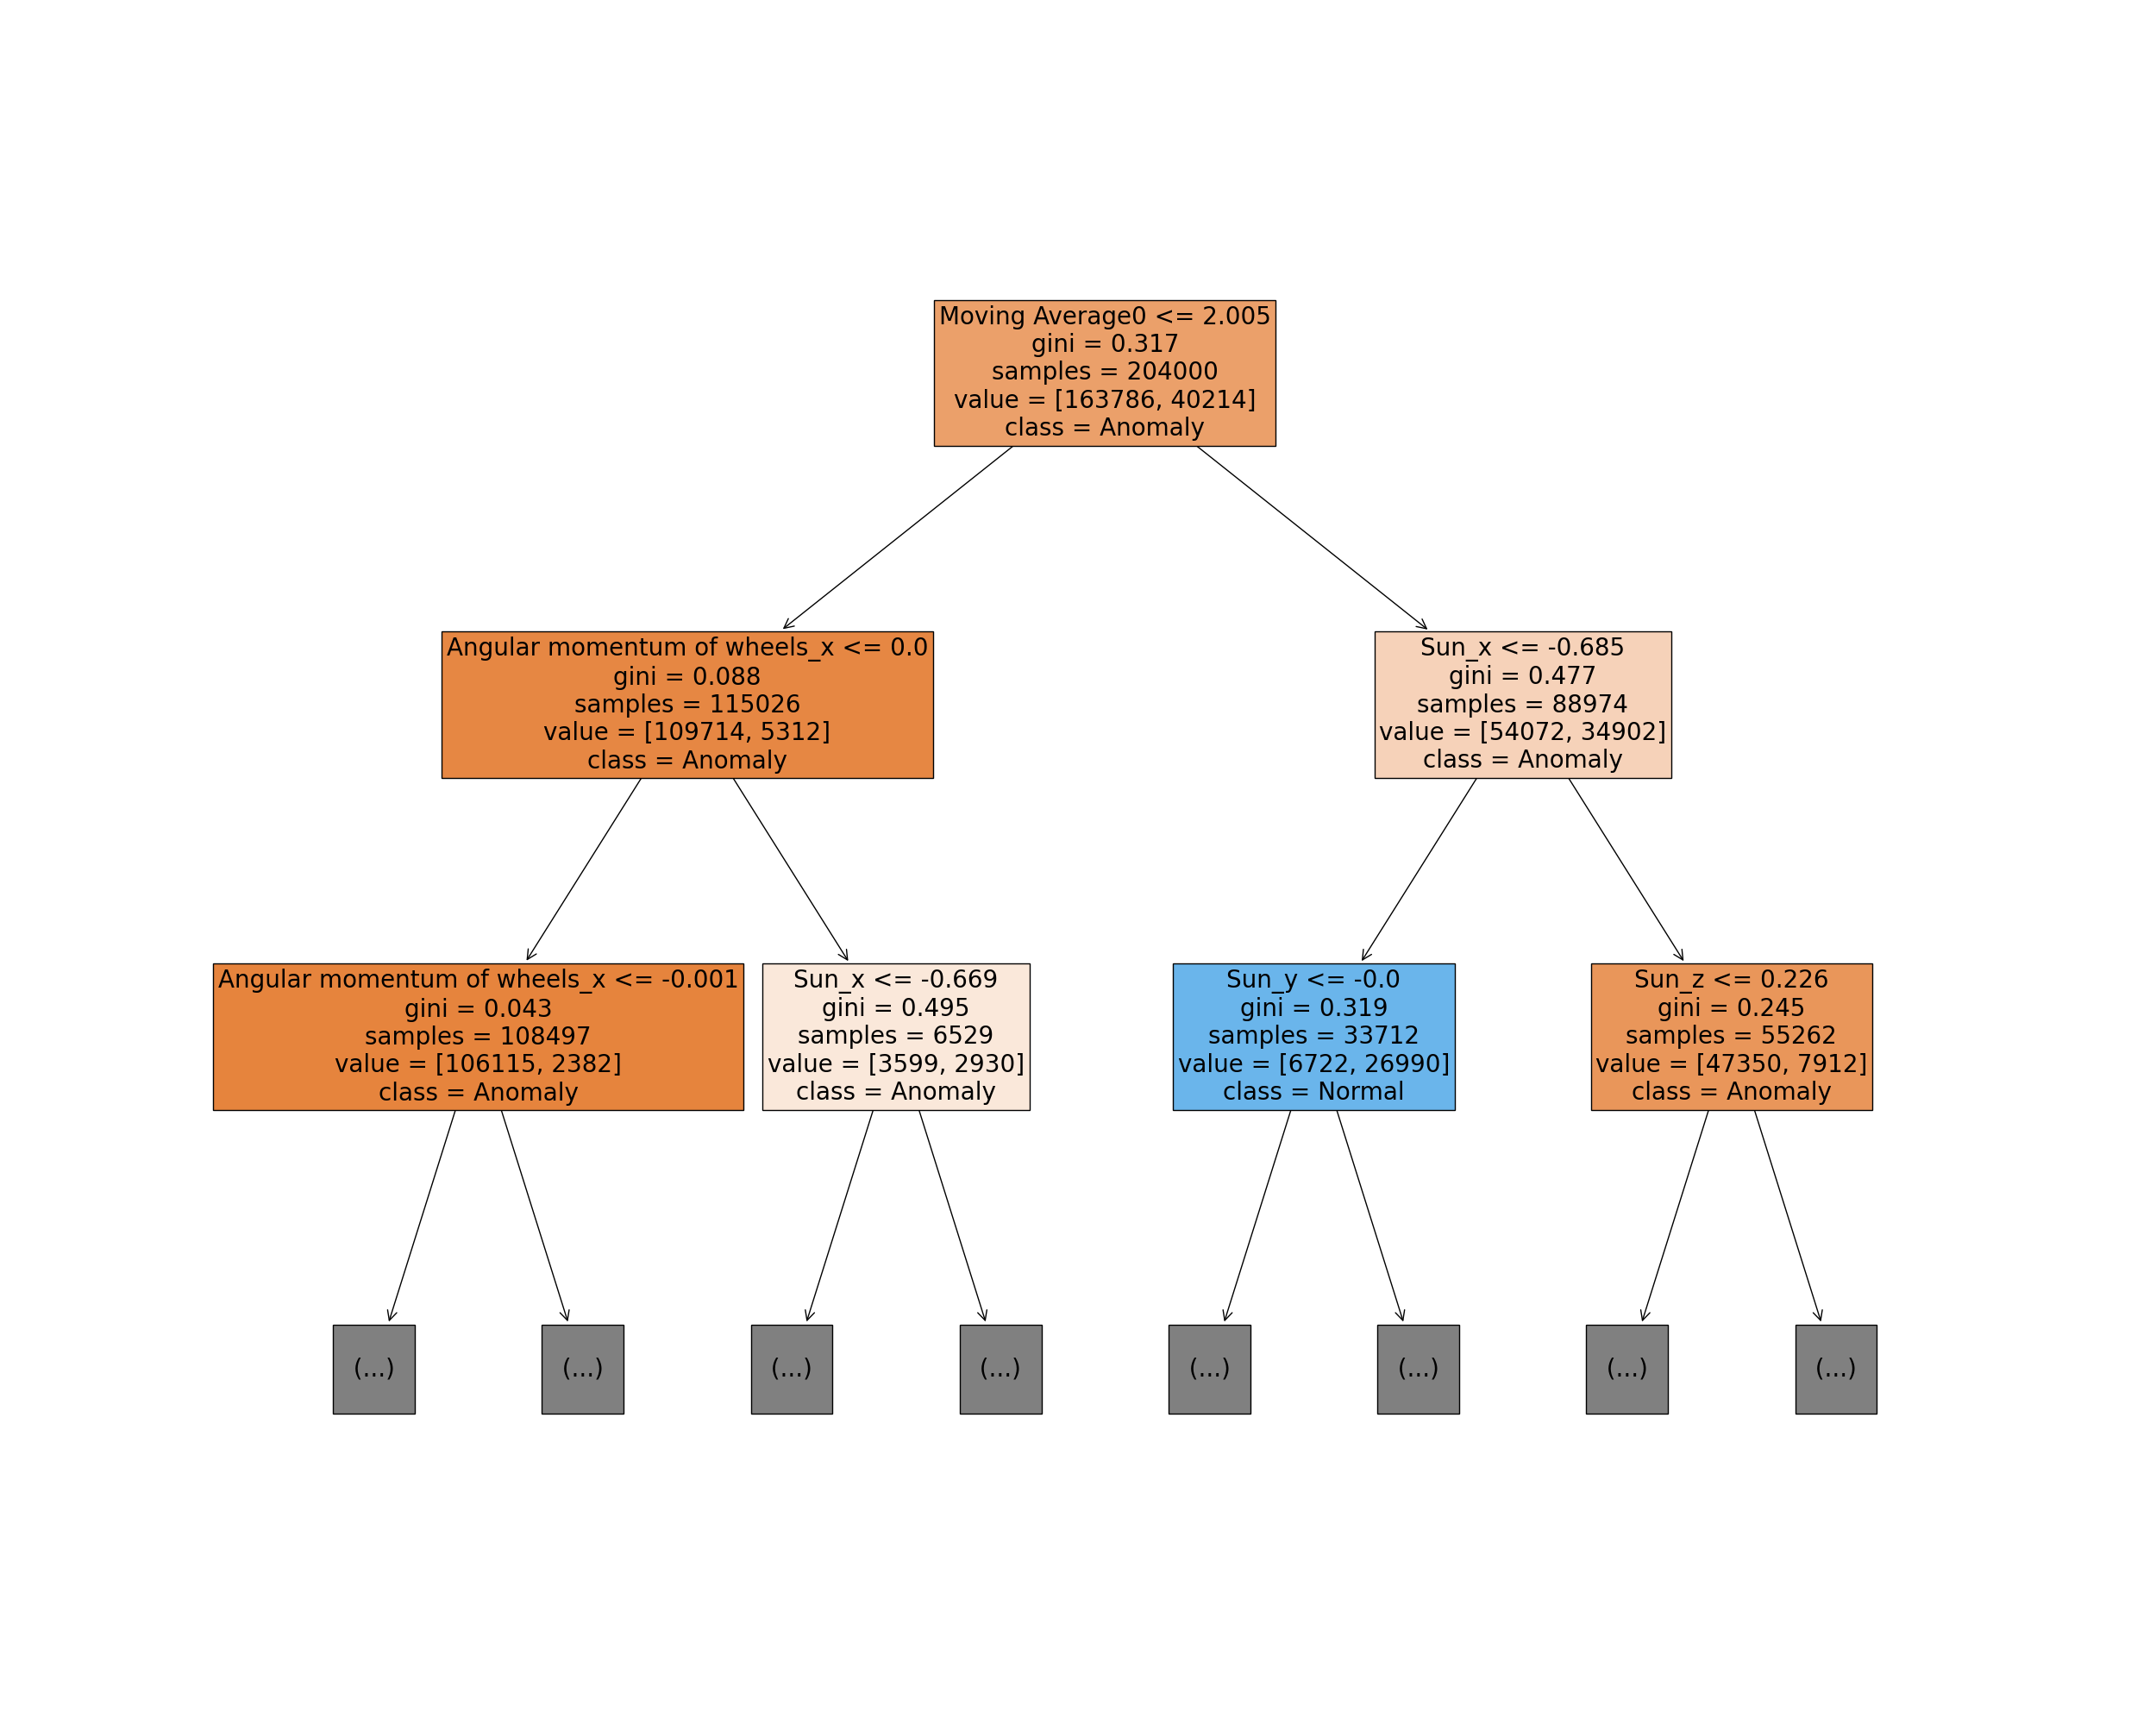
\includegraphics[trim = {4cm 8cm 4cm 8cm},clip, width = 15cm]{/home/ulrich/Documents/Masters thesis/Satellite/Hyperparameters/PhysicsEnabledDMDMethod/DecisionTreeBinaryClass.png}
%	\caption{Decision Tree}
%	\label{fig:DecisionTree}
%\end{figure*}

It is evident in Figure~\ref{fig:DecisionTree} that the most notable splits at the beginning of the tree are the moving average from the feature extraction as well as the sun sensor and angular momentum of the reaction wheels measurements. This makes logical sense since the moving average provides the system with an extracted feature that correlates with the change in measurements. The sun reflection can also be detected on the sun sensor measurements, and changes in the angular momentum of the wheels indicate that there could be significant changes in the sun vector during the sun following period.

Random forests, a method of using the prediction average of randomly sampled decision trees, is also tested, and the results thereof are shown in section~\ref{section:Results}.


\subsection{Recovery}
Three different methods of recovery are compared. These methods are all focused on ensuring that the sun reflection does not change the reliability and stability of the EKF.

The ignore method uses the detected sensor that has failed and ignores the sensor measurement from the EKF measurement update. This method is based on the assumption that the EKF estimation is correct up until the moment where the sensor failure is detected. This, however, will highly depend on the accuracy of the anomaly detection method. Since a detection method with low accuracy will create instability of the EKF since many anomalous measurements will be included in the measurement update of the EKF.

%The replacement methodology changes $v_{meas,k}$ to $v_{est,k}$ at the timestep when the failure is detected. This method depends on the stability and accuracy of the EKF when the failure is detected and highly depends on the accuracy of the detection method. However, this seems to bypass the entire purpose of a measurement update and might change the EKF's dependency to be more on the sensor than the model, even though the sensor measurement might not be accurate. The EKF will remain stable due to the other measurements being accurate and will save computation time. The EKF will not require any reset, and the same number of measurements updates will still occur during a sensor's anomalous behaviour.

The backtrack method uses a buffer of $v_{meas,k}$, $v_{model,k}$ and $\hat{x}_k^+$ and other parameters that are used to update the EKF. If a sensor failure is detected, the sensor is excluded from the EKF, and the EKF is updated with the sensor data in the buffer, excluding the sensor that has failed. The EKF is, therefore, \emph{reset} and updated from timestep $t_{k-N}$ to $t_k$, where $N$ is the size of the number of timesteps in the buffer. $N$, however, must be optimised based on the computational time used to reset the EKF but still ensure convergence of the EKF. If the sensor that was detected to have anomalous behaviour changes back to normal again, the EKF will be reset once again, and the sensor will only be included in the measurement update of $t_k$ since it was anomalous for timesteps before $t_k$.

A backtracking method can be combined with the ignore method. For example, where the backtracking method is implemented only after a specified number of sun reflections are predicted.

Another method implemented and tested always uses the two sensors measurements that have the smallest mean squared error between the estimated SBC vector and the actual measured SBC vector. There are setbacks to this method. Firstly, it requires the modelling of the ORC vector and requires the position of the satellite in orbit. Secondly, this method will not work with small drifts in a sensor measurement since the estimator will latch unto the drift in the sensor. The method will only detect sudden changes in the sensor and isolate the sudden change even if it remains stable after the sudden change. This method will only be compared to the other methods as part of the analysis since the method is inherently different. The method is also used to aid the other methods during a period after an anomaly is detected.

\section{Testing Setup}
The sgp4 simulation environment is used for the positioning in orbit of the satellite to ensure repeatability of the tests conducted in this article. The disturbance torques modelled in this simulation is the aerodynamic disturbances, static and dynamic wheel disturbances, gravity gradient disturbances, and gyroscopic disturbances. The testing for the FDIR methods is done by implementing a reflection model on a CubeSat from the moment of launching the satellite. Therefore the recovery methods are also implemented from the beginning of the satellite orbit. The mission of the ADCS of this specific satellite is to be nadir pointing during eclipse and sun following otherwise.

\subsection{Control}
Quaternion-feedback control with momentum dumping is only implemented during an eclipse. The attitude command vector during nadir-pointing in the SBC frame is $\mathbf{u}_c = [0, 0, 1]$, since the SBC frame $z$ coordinate should line up with the ORC frame. During the sun following phase, the attitude command according to \textcite{chen2000ground} can be calculated as 

\begin{equation}
\mathbf{u}_c = \frac{\mathbf{u}_{sp}^{SBC} \times \mathbf{s}_o}{\norm{\mathbf{u}_{sp}^{SBC} \times \mathbf{s}_o}}
\end{equation}

Where $\mathbf{s}_o$ is the measured unit sun vector in ORC, and the main solar panel's position is denoted as a unit vector, $\mathbf{u}_{sp}^{SBC}$. The angle between $\mathbf{u}_{sp}^{SBC}$ and $\mathbf{s}_o$, $\delta$, can be calculated with the vector dot-product. The command quaternion $\mathbf{q}_c$ can then be calculated

\begin{equation}
\mathbf{q}_c = \begin{bmatrix}
\mathbf{u}_c sin(\frac{\delta}{2}) \\
cos(\frac{\delta}{2})
\end{bmatrix}
\end{equation}
This can then be used as the reference for the control. The reference $\boldsymbol{\omega}_b^I$ is always $[0, 0, 0]$. The 

\subsection{Dimensions of Satellite}
The dimensions of the satellite are shown in Table~\ref{Table:Dimensions}. The dimensions are provided to ensure the repeatability of the results in this article. The dimensions of the sun sensor are from the Sputnix CubeSat sun sensor model.

\begin{table}[!htb]
	\caption{\label{Table:Dimensions}Dimensions of CubeSat}
	\begin{tabular}{|c|c|c|c|}
		\hline
		\textbf{Dimensions} & \textbf{Satellite (m)} & \textbf{Solar Panels (m)} & \textbf{Sun Sensor (m)} \\ \hline
		\textbf{x}          & $0.3$                    & $0.3$                       & $0.028$                   \\ \hline
		\textbf{y}          & $0.3$                    & $0.3$                       & $0.023$                   \\ \hline
		\textbf{z}          & $0.4$                    & $0.002$                     & N/A                     \\ \hline
	\end{tabular}
\end{table}

% https://sputnix.ru/en/equipment/CubeSat-devices/sun-sensor-flight-proof-1
% https://www.CubeSatshop.com/product/nss-CubeSat-sun-sensor/

\subsection{Orbit Parameters}
The orbit parameters will not significantly affect the results. However, for repeatability, the general parameters for the orbit are given in Table~\ref{Table:OrbitParameters}. 

\begin{table}[!htb]
	\caption{\label{Table:OrbitParameters}Parameters for CubeSat Orbit}
	\begin{tabular}{|c|c|}
		\hline
		\textbf{Revolutions per day}          & $15.2355$                    \\ \hline
		\textbf{Inclination}          & $97.4^o$                    \\ \hline
		\textbf{Right ascension of the ascending node} & $275^o$ \\ \hline
	\end{tabular}
\end{table}

\subsection{Sensors}
The measurement update of the Kalman filter will firstly be with a magnetometer, nadir sensor and lastly, the sun sensor. This is due to the noise models of the sensors, as all the sensor noise models are based on zero-mean Gaussian random noise, the magnetometer has the most significant standard deviation, and the sun sensor has the smallest standard deviation. There are two sun sensors, a coarse and fine sun sensor, which can experience sun reflection. The field of view \emph{FOV} of the sun sensors and the nadir sensor are both $180^o$. There is, however, only a single nadir sensor used in the simulation.

\section{Results}
\label{section:Results}
Three scenarios are implemented, a satellite that never experience reflection, a satellite that experiences reflection without any recovery method and a satellite with a recovery method. The subsets of detecting and recovering from the fault will be isolated and discussed separately. Therefore the results for recovery based on perfect detection can be shown to provide the theoretical possibilities of the recovery method. Please note that the scale of the y-axis for each plot is not the same due to the significant differences between the maximum y-values for each scenario.

The pointing metric is the difference between the command or reference attitude and the actual attitude in degrees. The estimation metric is the difference between the actual and estimated attitudes in degrees.

\subsection{Perfect Designed Satellite Without Reflection}
This test is implemented for the current design, assuming that the sun sensor will never experience sun reflection. This also indicates the best scenario for the ADCS and requires a well-designed satellite. The results for the first $5$ orbits are shown to provide a desired result for the recovery methods as shown in Figure~\ref{fig:Pointing Accuracy None} and Figure~\ref{fig:Estimation Accuracy None}. 
\begin{figure}[!htb]
	\begin{center}
		\import{Figures/TexFigures/Predictor-None/Isolator-None/Recovery-None/EARTH_SUN-ORC-General CubeSat Model/None/}{Pointing Metric.pgf}
	\end{center}
	\caption[Pointing Metric for Satellite Without Reflection]{Pointing Metric for Satellite Without Reflection.}
	\label{fig:Pointing Accuracy None}
\end{figure}

\begin{figure}[!htb]
	\begin{center}
		\import{Figures/TexFigures/Predictor-None/Isolator-None/Recovery-None/EARTH_SUN-ORC-General CubeSat Model/None/}{Estimation Metric.pgf}
	\end{center}
	\caption[Estimation Metric for Satellite Without Reflection]{Estimation Metric for Satellite Without Reflection.}
	\label{fig:Estimation Accuracy None}
\end{figure}

Figure~\ref{fig:Pointing Accuracy None} shows the transition of the reference vector between the eclipse and sunlit phases. This is the reason for the spikes in the pointing metric at the beginning of each period. From Figure~\ref{fig:Estimation Accuracy None} it is also evident that the estimation is more accurate during the sunlit phase, which correlates with the fact that the sun sensor has a smaller noise.

\subsection{Satellite With Reflection}
If no recovery strategy is implemented for the reflection anomaly, the EKF is unstable, and the estimation is inaccurate. As a bare minimum, the proposed methods should lower the estimation metric as shown in Figure~\ref{fig:Estimation Accuracy Reflection} of which the average estimation metric per orbit is also indicated in Figure~\ref{fig:Estimation Metric Summary}. It is clear that the ADCS is unstable due to sun reflection.

\begin{figure}[!htb]
	\begin{center}
		\import{Figures/TexFigures/Predictor-None/Isolator-None/Recovery-None/EARTH_SUN-ORC-General CubeSat Model/Reflection/}{Estimation Metric.pgf}
	\end{center}
	\caption[Estimation Metric for Satellite with Reflection and without FDIR]{Estimation Metric for Satellite with Reflection and without FDIR.}
	\label{fig:Estimation Accuracy Reflection}
\end{figure}

\subsection{Perfect Detection}
This section provides the results for each recovery method, with the assumption that the detection method is perfect. This means that the detection methodology will produce an accuracy of $100\%$. This is used to determine which method is most suitable for recovery from sensor anomalies since it provides the theoretical best scenario for each method. The mean estimation for each orbit is shown in Figure~\ref{fig:Estimation Metric Summary}, and it is evident that the EKF-ignore method is the method that reduces the estimation error the most during a period of $30$ orbits. 

\begin{figure}[!htb]
	\begin{center}
		\import{Figures/TexFigures/Summary/PERFECT/}{Estimation Metric.pgf}
	\end{center}
	\caption[Estimation Metric for Perfect Detection]{Estimation Metric for Perfect Detection.}
	\label{fig:Estimation Metric Summary}
\end{figure}

Due to the significant difference in performance between the EKF-ignore and the other recovery methods, only the EKF-ignore method will be further investigated with other detection strategies. The estimation metric for the EKF-ignore provides an average of $3.43^o$ per orbit.

\subsection{Satellite With Recovery Ignore}
To show the promising results of the recovery ignore for perfect detection, Figure~\ref{fig:Estimation Accuracy EKF-ignore} shows the estimation metric during the first five orbits. Our goal is to introduce detection strategies that produce similar results.

\begin{figure}[!htb]
	\begin{center}
		\import{Figures/TexFigures/Predictor-PERFECT/Isolator-OnlySun/Recovery-EKF-ignore/EARTH_SUN-ORC-General CubeSat Model/Reflection/}{Estimation Metric.pgf}
	\end{center}
	\caption[Estimation Metric for Satellite with Recovery Ignore]{Estimation Metric for Satellite with Recovery Ignore.}
	\label{fig:Estimation Accuracy EKF-ignore}
\end{figure}

To analyse what is required from the detection strategies to produce acceptable results, we perform a few tests with fixed percentage accuracies. This analysis is done by performing uniform randomness with the fixed accuracy percentage. Firstly we test the fixed accuracies by performing prediction on reflection and no reflection time steps. Therefore there can be both false positives and false negatives. The results, therefore, are shown in Figure~\ref{fig:Estimation Accuracy EKF-ignore Comparison}.

\begin{figure}[!htb]
	\begin{center}
		\import{Figures/TexFigures/Summary/EKF-ignore/}{Estimation MetricComparison-Standard.pgf}
	\end{center}
	\caption[Estimation Metric of Fixed Percentage Accuracies During Failures and No Failures]{Estimation Metric of Fixed Percentage Accuracies During Failures and No Failures.}
	\label{fig:Estimation Accuracy EKF-ignore Comparison}
\end{figure}

It is evident in Figure~\ref{fig:Estimation Accuracy EKF-ignore Comparison} that the percentage accuracy to produce an estimation metric average of less than $20^o$ per orbit is $99\%$. This is a challenging task to accomplish. Therefore, we want to determine the effects of perfect prediction during no reflection time steps. We perform a test where the prediction is only performed when reflection occurs, and during no reflection, a $100\%$ accuracy is used. The results, therefore, is shown in Figure~\ref{fig:Estimation Accuracy EKF-ignore Comparison PerfectNoFailure}, which indicates that the most significant effect on the EKF's estimation accuracy is not false negatives, but false positives.

\begin{figure}[!htb]
	\begin{center}
		\import{Figures/TexFigures/Summary/EKF-ignore/}{Estimation MetricPerfectNoFailurePrediction.pgf}
	\end{center}
	\caption[Estimation Metric of Fixed Percentage Accuracies During Failures and Perfect Prediction During No Failures]{Estimation Metric of Fixed Percentage Accuracies During Failures and Perfect Prediction During No Failures.}
	\label{fig:Estimation Accuracy EKF-ignore Comparison PerfectNoFailure}
\end{figure}

Therefore, we want to make sure that more failures are accurately predicted. Therefore, we want to implement a first-order filter after a failure is predicted to reduce the number of incorrectly predicted reflections. This, however, cannot be done by just ignoring the sun vector for some time since this will reduce the accuracy.

\subsection{First Order Filter}
\label{section:First Order Filter}
A method that only uses the two sensors whose measurement is the closest to the estimated vectors from the EKF for the measurement update is implemented. This method will be named EKF-top2 for ease of reference. The results of this method are shown in Figure~\ref{fig:Estimation Accuracy EKF-top2 summary}. The average estimation error is reduced to less than $20^o$. This method will consequently be used during a specific period after a failure is predicted. However, it cannot be used continually since the overall accuracy is reduced by only using $2$ sensors and assuming that there is always a failure.

\begin{figure}[!htb]
	\begin{center}
		\import{Figures/TexFigures/Summary/EKF-top2/}{Estimation Metric.pgf}
	\end{center}
	\caption[Estimation Metric for Satellite with Recovery Ignore and Various detection Methods]{Estimation Metric for Satellite with Recovery Ignore and Various Detection Methods.}
	\label{fig:Estimation Accuracy EKF-top2 summary}
\end{figure}

Now we want to test what the estimation error is for various fixed accuracy percentages with the EKF-ignore method and then implement the EKF-top2 method during the buffer period. We firstly conduct the test for various time steps during which the EKF-top2 must be performed at a constant accuracy of $90\%$ for which the results are shown in Figure~\ref{fig:Prediction Accuracy 90.0 with various steps summary}. 

\begin{figure}[!htb]
	\begin{center}
		\import{Figures/TexFigures/Summary/90.0/}{Estimation Metric.pgf}
	\end{center}
	\caption[Estimation Metric of $90.0\%$ Accuracy with Various Time Delays]{Estimation Metric of $90.0\%$ Accuracy with Various Time Delays.}
	\label{fig:Prediction Accuracy 90.0 with various steps summary}
\end{figure}

From Figure~\ref{fig:Prediction Accuracy 90.0 with various steps summary} the buffer period is selected as $10$ time steps after a failure is detected. The results thereof are shown in Figure~\ref{fig:Estimation Accuracy EKF-ignore with Recovery Buffer} for a range of realistic accuracies as expected from the various detection strategies. 

\begin{figure}[!htb]
	\begin{center}
		\import{Figures/TexFigures/Summary/10/}{Estimation Metric10Depths.pgf}
	\end{center}
	\caption[Estimation Metric of Fixed Percentage Accuracies During Failures and No Failures with Recovery Buffer]{Estimation Metric of Fixed Percentage Accuracies During Failures and No Failures with Recovery Buffer.}
	\label{fig:Estimation Accuracy EKF-ignore with Recovery Buffer}
\end{figure}

The required percentage accuracy is lowered dramatically with the first order filter implementation. Percentage accuracy of $70.0\%$ with the first order filter is performing similarly to a $99.5\%$ accuracy without the buffer after $10$ orbits. After we have now analysed the results for various fixed accuracies and the first order filter, we can now implement the detection methods with the recovery methods and determine the efficiency of the detection methods.

\subsection{Detection Methods}
Firstly, we want to analyse how the maximum root depth for both random forest and decision trees changes the accuracy of the detection strategies. In Table~\ref{Table: Prediction Accuracy-DMDRandomForestOnlySunEKF-ignoreReflection-Reflection} the false and true positives and false and true negatives are shown in the confusion matrices for different depths. It is clear from the average of the false positive and false negative that a depth of $20$ is the best for the random forest. This is also chosen instead of a $100$ since a depth of a $100$ is computationally much more expensive than a depth of $20$.

\begin{table*}
	\caption{Confusion Matric for RandomForest} 
	\label{Table: Prediction Accuracy-DMDRandomForestOnlySunEKF-ignoreReflection-Reflection} 
	\centering
	\begin{minipage}[c]{0.2\textwidth}
		\import{Tables/Prediction Accuracy/}{Prediction Accuracy-DMDRandomForest5OnlySunEKF-ignoreReflection-Reflection.tex}
		\subcaption{Depth of 5}
	\end{minipage}
	\begin{minipage}[c]{0.2\textwidth}
		\import{Tables/Prediction Accuracy/}{Prediction Accuracy-DMDRandomForest10OnlySunEKF-ignoreReflection-Reflection.tex}
		\subcaption{Depth of 10}
	\end{minipage}
	\begin{minipage}[c]{0.2\textwidth}
		\import{Tables/Prediction Accuracy/}{Prediction Accuracy-DMDRandomForest20OnlySunEKF-ignoreReflection-Reflection.tex}
		\subcaption{Depth of 20}
	\end{minipage}
	\begin{minipage}[c]{0.2\textwidth}
		\import{Tables/Prediction Accuracy/}{Prediction Accuracy-DMDRandomForest100OnlySunEKF-ignoreReflection-Reflection.tex}
		\subcaption{Depth of 100}
	\end{minipage}
\end{table*}

For the decision tree the confusion matrices are shown in Table~\ref{Table: Prediction Accuracy-DMDDecisionTreesOnlySunEKF-ignoreReflection-Reflection}. Although the lowest false negatives are at a depth of $5$, the false positive is significantly higher than a depth of $10$ and $15$. This essentially means that there are multiple instances where a failure will be predicted while there is no failure. Comparing the depth of $10$ and $20$, the sum of the false positive and false negatives are $211$ more at a depth of $20$. However, false negatives are more concerning than false positives, and from a depth of $10$ to a depth of $20$, the false negatives decrease by $4494$. The depth of $100$ has too many false positives for the small decrease of false negatives, and consequently, the depth of $20$ is used.

\begin{table*}[h!tb]
	\caption{Confusion Matric for Decision Trees} 
	\label{Table: Prediction Accuracy-DMDDecisionTreesOnlySunEKF-ignoreReflection-Reflection} 
	\centering
	\begin{minipage}[c]{0.2\textwidth}
		\import{Tables/Prediction Accuracy/}{Prediction Accuracy-DMDDecisionTrees5OnlySunEKF-ignoreReflection-Reflection.tex}
		\subcaption{Depth of 5}
	\end{minipage}
	\begin{minipage}[c]{0.2\textwidth}
		\import{Tables/Prediction Accuracy/}{Prediction Accuracy-DMDDecisionTrees10OnlySunEKF-ignoreReflection-Reflection.tex}
		\subcaption{Depth of 10}
	\end{minipage}
	\begin{minipage}[c]{0.2\textwidth}
		\import{Tables/Prediction Accuracy/}{Prediction Accuracy-DMDDecisionTrees20OnlySunEKF-ignoreReflection-Reflection.tex}
		\subcaption{Depth of 20}
	\end{minipage}
	\begin{minipage}[c]{0.2\textwidth}
		\import{Tables/Prediction Accuracy/}{Prediction Accuracy-DMDDecisionTrees100OnlySunEKF-ignoreReflection-Reflection.tex}
		\subcaption{Depth of 100}
	\end{minipage}
\end{table*}

Using the depth of $20$ for both random forest and decision trees, we determine the average estimation error for $30$ orbits with and without the first order buffer of $10$ time steps as shown in Figure~\ref{fig:Estimation Accuracy EKF-ignore DT and RF} and Figure~\ref{fig:Estimation Accuracy EKF-ignore DT and RF with Recovery Buffer}. It is clear that the first order buffer implementation increases the estimation error for the decision tree method but a slight decrease in the estimation error for the random forest. Comparing the prediction accuracy for both the decision tree and random forest, it is clear that both methods should at least produce better results than the theoretical $80$ accuracy. However, it is clear that they have higher estimation errors then the theoretical $80.0\%$. 

\begin{figure}[!htb]
	\begin{center}
		\import{Figures/TexFigures/Summary/EKF-ignore/}{Estimation MetricRF20DT20.pgf}
	\end{center}
	\caption[Estimation Metric of Decision Tree and Random Forest]{Estimation Metric of Decision Tree and Random Forest.}
	\label{fig:Estimation Accuracy EKF-ignore DT and RF}
\end{figure}

\begin{figure}[!htb]
	\begin{center}
		\import{Figures/TexFigures/Summary/EKF-ignore/}{Estimation MetricRF20DT20withBuffer.pgf}
	\end{center}
	\caption[Estimation Metric of Decision Tree and Random Forest with Recovery Buffer]{Estimation Metric of Decision Tree and Random Forest with Recovery Buffer.}
	\label{fig:Estimation Accuracy EKF-ignore DT and RF with Recovery Buffer}
\end{figure}

\begin{figure}[!htb]
	\begin{center}
		\import{Figures/TexFigures/Summary/EKF-ignore/}{Prediction AccuracyRF20DT20withBuffer.pgf}
	\end{center}
	\caption[Prediction Accuracy of Decision Tree and Random Forest with Recovery Buffer]{Prediction Accuracy of Decision Tree and Random Forest with Recovery Buffer.}
	\label{fig:Summary Prediction Accuracy EKF-ignore DT and RF with Recovery Buffer}
\end{figure}

To determine the behaviour of the detection strategies, we plot the prediction accuracy during the first $5$ orbits, but we do not plot the mean but the actual prediction accuracy. This is used to determine the time gaps between incorrect predictions, which would vary from the fixed accuracies. We isolate the random forest detection strategy for this analysis since it significantly outperforms the decision tree method.

From Figure~\ref{fig:Estimation Accuracy EKF-ignore DT and RF with Recovery Buffer} we see that the estimation metric for the first orbit is an average of $8.9^o$, which increases to $12.1^o$ in the second orbit, and by the $5^{th}$ orbit, the estimation error has increased to $20.8^o$. From Figure~\ref{fig:Prediction Accuracy EKF-ignore RF} and Figure~\ref{fig:Summary Prediction Accuracy EKF-ignore DT and RF with Recovery Buffer}, it is clear that there are two reasons for this increase in estimation error. Firstly, the average prediction accuracy decreases from $90\%$ during the first orbit to settle at an average of $86\%$. Secondly, the duration of inaccurate predictions increases, as seen in the horizontal line at $0$. These extensive durations of constant inaccurate prediction will increase the instability and decrease the accuracy of the EKF. These inaccurate predictions are due to the change of the satellite behaviour during recovery, which, in turn, influences the prediction. It is thus recommended to implement non-linear machine learning methods such as Support Vector Machines which will not produce single thresholds for each parameter but a kernel function that splits the data based on n-dimension planes.

%\begin{figure}[!htb]
%	\begin{center}
%		\import{Figures/TexFigures/Predictor-RandomForest20/Isolator-OnlySun/Recovery-EKF-ignore/EARTH_SUN-ORC-General CubeSat Model/ReflectionBufferValue-10BufferStep-0.9EKF-top2/}{Prediction Accuracy.pgf}
%	\end{center}
%	\caption[Prediction Accuracy of Decision Tree and Random Forest with Recovery Buffer]{Prediction Accuracy of Decision Tree and Random Forest with Recovery Buffer.}
%	\label{fig:Prediction Accuracy EKF-ignore RF}
%\end{figure}

\section{CONCLUSIONS}
It is clear from the analysis results that sun reflection recovery is possible with the proposed EKF-ignore method. It is also clear that the percentage accuracy for the detection is drastically decreased with a first-order buffer and the EKF-top2 method. However, both the decision tree and random forest method do not produce the desired results due to the decreased inaccuracy of the prediction after the recovery method is implemented. Therefore, it is recommended to further the testing with methods such as Support Vector Machines.

\addtolength{\textheight}{-12cm}   % This command serves to balance the column lengths
% on the last page of the document manually. It shortens
% the text height of the last page by a suitable amount.
% This command does not take effect until the next page
% so it should come on the page before the last. Make
% sure that you do not shorten the text height too much.

%%%%%%%%%%%%%%%%%%%%%%%%%%%%%%%%%%%%%%%%%%%%%%%%%%%%%%%%%%%%%%%%%%%%%%%%%%%%%%%%



%%%%%%%%%%%%%%%%%%%%%%%%%%%%%%%%%%%%%%%%%%%%%%%%%%%%%%%%%%%%%%%%%%%%%%%%%%%%%%%%

% \begin{thebibliography}{99}

% \bibitem{c1} G. O. Young, ÒSynthetic structure of industrial plastics (Book style with paper title and editor),Ó 	in Plastics, 2nd ed. vol. 3, J. Peters, Ed. New York:  % McGraw-Hill, 1964, pp. 15Ð64.
% \bibitem{c2} W.-K. Chen, Linear Networks and Systems (Book style).	Belmont, CA: Wadsworth, 1993, pp. 123Ð135.

\printbibliography[heading=bibintoc]




% \end{thebibliography}



\end{document}
